
\chapter{Il problema della ciclotomia}

In questo capitolo si trova una risposta al problema della ciclotomia, che può essere formulato con la seguente domanda: per quali $n \in \mathbb{N}$ è possibile costruire il poligono regolare di $n$ lati con riga e compasso?

%%%%%%%%%%%%%%%%%%%%%%%%%%%%%%%%
%%%%%%%%%%%%%%%%%%%%%%%%%%% SECTION 

\section{Poligoni regolari e numeri complessi}

Si considera l'insieme delle costruzioni euclidee, immerse nel piano di Gauss tramite
\begin{align*} \label{immersc}
\mathcal{I}_c:  \mathcal{E}(P_0,P_1) & \longrightarrow \mathbb{C} 
\end{align*}
che possiede caratteristiche analoghe a quelle di $\mathcal{I}$, funzione definita in \ref{immers}.
Si considerano i poligoni regolari nel piano complesso inscritti nella circonferenza unitaria centrata nell'origine e aventi un vertice nel punto $(1,0)$. In questo modo tutti i vertici di tali poligoni sono dati da potenze ennesime di numeri complessi e in particolare sono soluzioni di una equazione polinomiale.
Per verificare quanto affermato, si considerano da \cite{Rogg} le seguenti:

%% prop 1 da roggero
\begin{prop}(Potenze $n$-esime di un numero complesso) \label{potcompl}
Sia $z = (\rho, \theta)$ un numero complesso espresso in coordinate polari e sia $n \in \mathbb{N}$, allora $z^n = (\rho^n, n\theta)$
\end{prop}

\begin{prop}(Radici $n$-esime di un numero complesso) \label{radcompl}
Sia $z = (\rho, \theta)$ un numero complesso espresso in coordinate polari e sia $n \in \mathbb{N}$, allora l'equazione polinomiale $x^n - z = 0$ ha esattamente n soluzioni distinte le cui espressioni in coordinate polari sono 
\begin{align*} 
z_k = (\sqrt[n]{\rho} , \frac{\theta + 2k\pi}{n}) \qquad k = 0, 1, ... , n-1
\end{align*}
\end{prop}

Dalle proprietà appena enunciate, si deduce che, nella circonferenza unitaria le potenze $n$-esime di $z = (1, 0)$ (soluzioni di $x^n - 1 = 0$), sono date da 
\begin{align*} 
z_k = (1 , \frac{2k\pi}{n}) \qquad k = 0, 1, ... , n-1
\end{align*}
che geometricamente rappresentano i vertici di un poligono con $n$ lati inscritto nella circonferenza unitaria, avente un vertice in $(1,0)$.

Siano $\rho$ e $\theta$ coordinate polari del numero complesso $z$. Esso può essere rappresentato come $z = \rho \cos \theta + i \rho \sin \theta = (\rho, \theta)$, che equivale a $\rho e^{\theta i}$. Per rappresentare il $k$-esimo vertice di un poligono di $n$ lati, verrà utilizzata la seguente notazione:
\begin{align*} 
\delta_{n}^{k} := e^{\frac{2k\pi i}{n}} = \cos(\frac{2k\pi i}{n}) + i \sin(\frac{2k\pi i}{n}) =  (1 , \frac{2k\pi}{n})
\end{align*}
\noindent
che si avvale della formula di Eulero.

%%%%%% Osservazione radici n-esime
\begin{osservazione}
Il problema di costruire un poligono regolare di $n$ lati è equivalente al problema di costruire le soluzioni di $x^n - 1 = 0$. Infatti, come conseguenza della proprietà \ref{radcompl}, l'equazione polinomiale $x^n -1 = 0$ ha esattamente $n$ soluzioni distinte le cui espressioni in coordinate polari sono:
\begin{align*} 
\delta_{n}^{0} \quad \delta_{n}^{1} \quad \delta_{n}^{2} \phantom{z} \dots \phantom{z} \delta_{n}^{n-1} 
\end{align*}
Questa affermazione si dimostra considerando che $\delta_{n}^{j} \neq \delta_{n}^{k}$, per $j \neq k < n$, e che usando la formula delle potenze $n$-esime di un numero complesso si ottiene 
\begin{align*}
(\delta_{n}^{k})^n = (1^n, n\frac{2k\pi i}{n}) = (1,0) = 1 
\end{align*}
\end{osservazione}

%%%%%%%%%%%%%%%%%%%%
%%%%%%%%%%%%%%%%%%%%%%%%%% SECTION Estensioni ciclotomiche

\section{Radici $n$-esime dell'unità ed estensioni ciclotomiche}
In questo paragrafo si vuole stabilire per quali $n$ il numero complesso $\delta_{n}^{1}$ è euclideo.
Se il secondo vertice $\delta_{n}^{1}$ di un poligono di $n$ lati è euclideo, allora il lato del poligono è costruibile e quindi la costruzione di tale poligono è immediata.
Dal corollario \ref{corolla} si ha che se $\delta_{n}^{1} \in \mathbb{C}$ è euclideo, allora $\delta_{n}^{1}$ è algebrico di grado $2^k$ per un opportuno naturale k. E' quindi necessario studiare il grado dell'estensione in cui si trova $\delta_{n}^{1}$.

%%% DEFINIZIONE radici n-esime dell'unità, ordine, radici primitive
\begin{definizione}
Le radici del polinomio $x^n - 1$ sono dette \begin{bfseries}radici $n$-esime dell'unità\end{bfseries} e si indicano con $\delta_{n}^{k}$ per $1\leq k \leq n-1$. Si definisce \begin{bfseries}ordine\end{bfseries} o \begin{bfseries}periodo\end{bfseries}, di una radice $n$-esima dell'unità $\delta_{n}^{k}$ il più piccolo intero positivo $m$ tale che $(\delta_{n}^{k})^m = 1$. Inoltre una radice $n$-esima dell'unità $\delta_{n}^{k}$ si dice \begin{bfseries}primitiva\end{bfseries}, se il suo ordine è $n$, cioè $(\delta_{n}^{k})^n = 1$. 
\end{definizione}

%% OSSERVAZIONE quante radici primitive ci sono?
\begin{osservazione}
Ci sono esattamente $\phi(n)$ radici $n$-esime primitive dell'unità, dove $\phi$ è la funzione di Eulero. Infatti $(\delta_{n}^{k})^m = 1$ se e solo se $(m,k) = 1$. Se ci fossero divisori comuni fra $m$ e $k$, allora $m$ non sarebbe più il più piccolo intero positivo a cui elevare $\delta_{n}^{k}$ per ottenere $1$. Si osserva inoltre che $\delta_{n}^{1}$ è sempre radice $n$-esima dell'unità.
\end{osservazione}

%%%DEFINIZIONE estensione ciclotomica
\begin{definizione} 
Il campo di spezzamento del polinomio $x^n - 1$ su $\mathbb{Q}$ è detto \begin{bfseries}estensione ciclotomica\end{bfseries}. Si indica con $\mathbb{Q}(\delta_{n}^{k})$ per $\delta_{n}^{k}$ radice primitiva $n$-esima dell'unità.
\end{definizione}

%% OSSERVAZIONE grado dell'estensione ciclotomica
\begin{osservazione} \label{osservazionedue}
Dato che ci sono esattamente $\phi(n)$ radici $n$-esime primitive dell'unità, l'estensione ciclotomica  ha grado $\phi(n)$. Cioè
\begin{align*} 
[\mathbb{Q}(\delta_{n}^{k}): \mathbb{Q}] = \phi(n)
\end{align*}
\end{osservazione}

%Mini storia
Il prossimo teorema comincia a far intravedere per quali fattorizzazioni di $n$ i poligoni regolari di $n$ lati sono costruibili; sarà poi nell'ultimo teorema del paragrafo, la cui condizione necessaria fu dimostrata da Gauss nel 1801 e la condizione sufficiente da Pierre Laurent Wantzel nel 1836\footnote{Da \cite{kline} pag. 879}, che si avrà un criterio effettivo per rispondere al problema della ciclotomia.

%%TEOREMA Sulla costruibilità per phi
\begin{teorema}\footnote{Da \cite{cattaneo}, corollario $7.5.2$ pag. 375 .} \label{teoremaprimo}
Un poligono regolare di $n$ lati è costruibile se e solo se esiste un intero positivo $h$ tale che $\phi(n) = 2^h$
\end{teorema}

\begin{proof}
Il poligono di $n$ lati e costruibile se e solo se $\delta_{n}^{1}$ è costruibile; per \ref{tfond}, esiste $h \in \mathbb{N}$ tale che 
\begin{align*} 
[\mathbb{Q}(\delta_{n}^{1}): \mathbb{Q}] = 2^h
\end{align*}
E per \ref{osservazionedue} segue che
\begin{align*} 
[\mathbb{Q}(\delta_{n}^{1}): \mathbb{Q}] = \phi(n)
\end{align*}
Cioè $\phi(n) = 2^h$.
\\\\
Viceversa, se vale $\phi(n) = 2^h$, allora dall'osservazione \ref{osservazionedue} segue che
\begin{align*} 
[\mathbb{Q}(\delta_{n}^{1}): \mathbb{Q}] = \phi(n) = 2^h
\end{align*}
Quindi $\delta_{n}^{1}$ è un punto euclideo. Pertanto è euclideo anche il lato del poligono di $n$ lati.
\end{proof}

% LEMMA PRIMO SU PHI
\begin{lemmax}\footnote{Da \cite{cattaneo}, proposizione $2.8.3$ pag. 85 .} \label{lemmaprimo}
Se $p$ è un numero primo allora $\phi(p^h) = p^h - p^{h-1}$
\end{lemmax}

\begin{proof}
Non sono coprimi con $p^h$ solo i multipli di $p$, quindi solo gli elementi $i \cdot p$, per $1 \leq i \leq h-1$. La cardinalità degli elementi non coprimi con $p^h$ è quindi $h-1$, cioè $\phi(p^h) = p^h - p^{h-1}$.
\end{proof}

%% LEMMA SECONDO SU PHI
\begin{lemmax}\footnote{Da \cite{cattaneo}, proposizione $2.9.7$ pag. 93 .}\label{lemmasecondo}
Condizione necessaria (ma non sufficiente) affinché un numero della forma $2^h + 1$ sia primo è che l'esponente deve avere la forma $h = 2^k$ per qualche k intero positivo.
\end{lemmax}

\begin{proof}
Se per assurdo $h$ contiene un fattore dispari, cioè $h = r(2s+1)$ per $r$ ed $s$ interi positivi, allora 
\begin{align*} 
2^h + 1& = 2^{r(2s+1)} +1 \\
& = (2^r +1)((2^r)^{2s} - (2^r)^{2s-1} + (2^r)^{2s-2} - \dots + (2^r)^{2} - 2^r + 1)
\end{align*}
si separa nel prodotto di due fattori. Non vale la condizione sufficiente (Eulero 1732), infatti
\begin{align*}  
2^{2^{5}} + 1 = 4294967297 = 641 \cdot 6700417
\end{align*}
\end{proof}


%%%%%%%%%%%%%%%% TEOREMONE DI FINE PARAGRAFO SULLA SOLUZIONE DEL PROBLEMA DELLA CICLOTOMIA
\begin{teorema}\footnote{Da \cite{cattaneo}, proposizione $7.5.3$ pag. 375. } \label{teoremaciclotomia}
Un poligono di $n$ lati è costruibile se e solo se i primi dispari che compaiono nella fattorizzazione hanno tutti esponente $1$ e sono primi del tipo $2^{2^{n}} +1$. Cioè la fattorizzazione di n è del tipo
\begin{align*} 
n = 2^k p_1 p_2 \dots p_s
\end{align*}
con $p_1 p_2 \dots p_s$ numeri distinti del tipo $2^{2^{n}} +1$.
\end{teorema}

\begin{proof}
Da \ref{teoremaprimo} si ha che un poligono regolare di $n$-lati è costruibile $\Leftrightarrow  \exists h \in \mathbb{N} \mid  \phi(n) = 2^h$. Sia $n = p_{1}^{t^1} p_{2}^{t^2} \dots p_{r}^{t^r}$ per $p_{i}$ primo, e $t^i$ intero positivo, allora da \ref{lemmaprimo}
\begin{align*} 
\phi(n) & = \phi(p_{1}^{t^1}) \phi( p_{2}^{t^2}) \dots \phi(p_{r}^{t^r}) \\
& = (p_{1}^{t^1} - p_{1}^{t^1 -1})(p_{2}^{t^2} - p_{2}^{t^2 -1}) \dots (p_{r}^{t^r} - p_{r}^{t^r -1})
\end{align*}
Ora per poter affermare che $\phi(n) = 2^h$, si deve stabilire quando il generico fattore $(p^{k} - p^{k -1})$ è una potenza di $2$. Si osserva che ciò accade solo in due casi: per $p = 2$ e per ogni $k$ intero positivo oppure, se $p \neq 2$, per $k = 1$ e $p - 1 = 2^t$. Ovvero 
\begin{enumerate}
\item $(p^{k} - p^{k -1}) = (2^{k} - 2^{k -1}) = 2^{k-1}(2-1) = 2^{k-1}$

\item $(p^{k} - p^{k -1}) = (p^{1} - 1) = 2^{t}$

\end{enumerate}

Se tutti i fattori $(p^{k} - p^{k -1})$ sono del tipo $1$, allora $\phi(n) = 2^{k-1}$.
Se tutti i fattori $(p^{k} - p^{k -1})$ sono del tipo $2$, allora tali fattori sono del tipo $p-1 = 2^t$, cioè $p = 2^t + 1$ per p che deve essere primo. Per  \ref{lemmasecondo} $p$ è primo se e solo se è del tipo $2^{2^m} + 1$.
Nel caso generico, in cui i fattori di $n$ possono essere sia del tipo $1$ che del tipo $2$, si ha che
\begin{align*} 
n = 2^k p_1 p_2 \dots p_s
\end{align*}
con $p_1 p_2 \dots p_s$ numeri distinti del tipo $2^{2^{n}} +1$.
\end{proof}

\noindent
Dal teorema precedente si ottiene la seguente tabella:

\begin{center}
\begin{tabular}{c c c}
Numero di lati  & Fattorizzazione & Costruibilità \\
\hline
$3$  &  $2+1$  & sì \\
$4$  &  $2^2$  & sì \\
$5$  &  $2^2+1$  & sì \\
$6$  &  $2\cdot3$  & sì \\
$7$  &                 & no \\
$8$  &  $2^3$  & sì \\
$9$  &  $3\cdot3$  & no \\
$10$  &  $2\cdot5$  & sì \\
$11$  &                    & no \\
$12$  &  $2^2\cdot3$  & sì \\
$13$  &                  & no \\
$14$  &  $2\cdot7$  & no \\
$15$  &  $3\cdot5$  & sì \\
$16$  &  $2^4$  & sì \\
$17$  &  $2^4 + 1$  & sì \\
$18$  &  $2\cdot3^2$  & no \\
$19$  &                & no \\
$20$  &  $2^2\cdot5$  & sì \\
$21$  &  $3\cdot7$  & no \\
$22$  &  $2\cdot11$  & no \\
$23$  &                 & no \\
$24$  &  $2^3\cdot3$  & sì \\
$25$  &  $5^2$  & no \\
\hline
\end{tabular}
\end{center}

\noindent
Alla luce degli ultimi risultati, i numeri del tipo $2^{2^n} + 1$ assumono un'importanza particolare. Saranno approfonditi nel prossimo paragrafo.

%%%%%%%%%%%%%%%%%%%%%% SECTION
%%%%%%%%%%%%%%%%%%%%%% FERMAT

\section{Numeri di Fermat}

I numeri del tipo $F_n = 2^{2^{n}} +1$ sono detti numeri di Fermat, e prendono il nome dal matematico francese Pierre De Fermat (1601-1665).
\begin{align*}
n &= 0 &F_0 &= 3\\
n &= 1 &F_1 &= 5\\
n &= 2 &F_2 &= 17\\
n &= 3 &F_3 &= 257\\
n &= 4 &F_4 &= 65537 \\
& \vdots & \vdots
\end{align*}

Come già accenato nel capitolo precedente, non tutti i numeri di Fermat sono necessariamente primi. 
\\
Si sa che per $n = 6,7,8,9,11,12,18,23,36,38,73$, i corrispondenti numeri di Fermat non sono primi. Non è attualmente noto se esistano infiniti numeri di Fermat primi\footnote{Da \cite{Procesi} Osservazione $7.10$ di pag. $28$. }.

Vale il seguente teorema, dal quale segue una definizione ricorsiva dei numeri di Fermat.

\begin{teorema}\footnote{Da \cite{Kosh} Teorema $2.16$ di pag. $139$. }
Sia $F_n$ l'$n$-esimo numero di Fermat, allora, $F_n = F_{n-1}^2 - 2F_{n-1} + 2$ per $n \geq 1$.
\end{teorema}

\begin{proof}
Si verifica per sostituzione:

\begin{align*}
F_n & = F_{n-1}^2 - 2F_{n-1} + 2 \\
 & = (2^{2^{n-1}} +1)^2 - 2(2^{2^{n-1}} +1) + 2 \\
 & = (2^{2^{n}} + 2 \cdot 2^{2^{n-1}} +1) - 2 \cdot 2^{2^{n-1}} -2 + 2 \\
 & = 2^{2^{n}} +1\\
 & = F_n
\end{align*}
\end{proof}

\begin{definizione} (Ricorsiva)
I numeri che verificano la ricorsione
\begin{align*}
F_n &= 3\\
F_n &= F_{n-1}^2 - 2F_{n-1} + 2
\end{align*}
 sono detti \begin{bfseries}Numeri di Fermat\end{bfseries}.
\end{definizione}

Per scoprire quali fra i numeri di Fermat sono primi si riporta l'enunciato dell'interessante teorema di Pepin. Si omette la dimostrazione, che esula dallo scopo di questa tesi.

%%%%%%% Teorema di PEPIN
\begin{teorema}\footnote{Da \cite{Shanks} Teorema $55$ di pag. $119$. }
$F_n = 2^{2^{n}} +1$ è un numero primo se e solo se 
\begin{displaymath}
3^{\frac{F_{n} - 1}{2} }  \equiv 1 \quad  mod \phantom{z} F_{n}
\end{displaymath}
\end{teorema}

%%%%%%%%%%%%%%%%%%%%%% SECTION
%%%%%%%%%%%%%%%%%%%%% ESEMPI
\section{Alcuni esempi}

Si conclude il capitolo con gli esempi\footnote{Da \cite{sitowolfram}, \cite{sitoroi} e \cite{sito4}.  } della costruzione del decagono, del pentagono e dell'eptadecagono, indicati rispettivamente con $\Theta_{10}$, $\Theta_{5}$ e $\Theta_{17}$.

%%%%%%%%%%%%%%%%%%%%%%%%%%%%%%%%%%%%% PENTAGONO E DECAGONO
\subsection{Costruzione del decagono e del pentagono}  \label{decagono}

Si vuole costruire il decagono regolare inscritto nella circonferenza di centro $P_{0}$ e raggio $P_{0} P_{1}$, in modo che $P_{1}$ equivalga al primo vertice $\delta_{10}^{0}$. 

Si procede nel seguente modo:
\begin{enumerate}

\item Si tracci la costruzione $S_1$ di \ref{perp}, per ottenere le rette perpendicolari $R_{2}(P_{0}, P_{1})$ ed $R_{8}(P_{0}, P_{7})$.

\item Si evidenzi il punto $P_{9}(C_{3}, R_{8})$ e si costruisca $P_{14}$, punto medio del segmento $P_{0}P_{9}$, con la successione
\begin{align*}
&C_{10}(P_{9};\overline{P_{9} P_{0}}), P_{11}(C_{3}, C_{10}), P_{12}(C_{3}, C_{10}), \\
&R_{13}(P_{11}, P_{12}), P_{14}(R_{8}, R_{13})
\end{align*}

\item Si tracci la circonferenza $C_{15}(P_{14};\overline{P_{14} P_{0}})$ di centro $P_{14}$ e raggio $P_{14}P_{0}$. 

\item Si costruisca la retta $R_{16}(P_{1}, P_{14})$, che intercetta sulla circonferenza $C_{15}(P_{14};\overline{P_{14} P_{0}})$ il punto $P_{17}(C_{15}, R_{16})$.

\item Si tracci la circonferenza $C_{18}(P_{1};\overline{P_{1} P_{17}})$. Tale circonferenza interseca $C_{3}$ nel punto $P_{19}(C_{3},C_{18})$. Il punto appena costruito è $\delta_{10}^{1}$, secondo vertice del decagono regolare.

\item Ora che si ha il lato del decagono regolare $P_{0}P_{19}$, si costruiscono gli altri vertici del poligono con circonferenze successive di raggio pari al lato, con la seguente successione:
\begin{align*}
&C_{20}(P_{19};\overline{P_{19} P_{1}}), P_{21}(C_{3}, C_{20}) = \delta_{10}^{2}, C_{22}(P_{21};\overline{P_{21} P_{19}}), P_{23}(C_{3}, C_{22}) = \delta_{10}^{3}, \\
&C_{24}(P_{23};\overline{P_{23} P_{21}}), P_{25}(C_{3}, C_{24})= \delta_{10}^{4}, C_{26}(P_{25};\overline{P_{25} P_{23}}), P_{27}(C_{3}, C_{26})= \delta_{10}^{5}, \\
&C_{28}(P_{27};\overline{P_{27} P_{25}}), P_{29}(C_{3}, C_{28}) = \delta_{10}^{6}, C_{30}(P_{29};\overline{P_{29} P_{27}}), P_{31}(C_{3}, C_{30})= \delta_{10}^{7}, \\
&C_{32}(P_{31};\overline{P_{31} P_{29}}), P_{33}(C_{3}, C_{32})= \delta_{10}^{8}, C_{34}(P_{33};\overline{P_{33} P_{31}}), P_{35}(C_{3}, C_{34})= \delta_{10}^{9}
\end{align*}

\end{enumerate}

%%%%%%%%% IMMAGINE COSTRUZIONE DECAGONO %
\begin{figure}[!h]
%centrare
\begin{center}
\resizebox{12.7 cm}{9.5 cm}{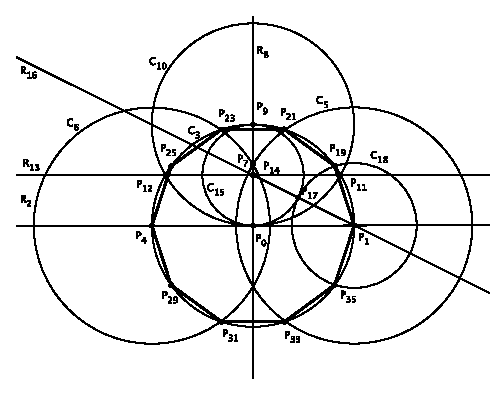
\includegraphics{3_decagon}} 
%\includegraphics{Decagono} 
\caption{Costruzione del decagono}
\end{center}
\end{figure}

Unendo i passaggi appena elencati, si ottiene la costruzione del decagono:
%%%%%%%%%%%%%%%%%%%%%%%%%%%%%%%%%%%%%%% Poly 10
\begin{align*}
\Theta_{10} =  & S_{1} \cup (P_{9}(C_{3}, R_{8}),  C_{10}(P_{9};\overline{P_{9} P_{0}}), P_{11}(C_{3}, C_{10}), \\
&P_{12}(C_{3}, C_{10}), R_{13}(P_{11}, P_{12}), P_{14}(R_{8}, R_{13})), C_{15}(P_{14};\overline{P_{14} P_{0}}) \\
& R_{16}(P_{1}, P_{14}), P_{17}(C_{15}, R_{16}), C_{18}(P_{1};\overline{P_{1} P_{17}}), P_{19}(C_{3},C_{18}) \\
&C_{20}(P_{19};\overline{P_{19} P_{1}}), P_{21}(C_{3}, C_{20}), C_{22}(P_{21};\overline{P_{21} P_{19}}), P_{23}(C_{3}, C_{22}), \\
&C_{24}(P_{23};\overline{P_{23} P_{21}}), P_{25}(C_{3}, C_{24}), C_{26}(P_{25};\overline{P_{25} P_{23}}), P_{27}(C_{3}, C_{26}), \\
&C_{28}(P_{27};\overline{P_{27} P_{25}}), P_{29}(C_{3}, C_{28}), C_{30}(P_{29};\overline{P_{29} P_{27}}), P_{31}(C_{3}, C_{30}), \\
&C_{32}(P_{31};\overline{P_{31} P_{29}}), P_{33}(C_{3}, C_{32}), C_{34}(P_{33};\overline{P_{33} P_{31}}), P_{35}(C_{3}, C_{34}))
\end{align*}

\noindent
Si ha che $\delta_{10}^{0} := P_{1} $ e $\delta_{10}^{k+1} := P_{19 + 2k}$ per $k = 0 \dots 8$.
\\
Per costruire il pentagono $\Theta_{5}$ è sufficiente considerare solo i vertici del tipo $\delta_{10}^{2k}$ per $k = 0 \dots 4 $ del decagono appena costruito.

%%%%%%%%%%%%%%%%%%%%%%%%%%%%%%% EPTADECAGONO
\subsection{Costruzione dell'eptadecagono}

Si propone la costruzione dell'eptadecagono regolare inscritto nella circonferenza di centro $P_{0}$ e raggio $P_{0} P_{1}$, in modo che $P_{1}$ equivalga al primo vertice $\delta_{17}^{0}$:

\begin{enumerate}
% 1
\item Si tracci la costruzione $S_1$ di \ref{perp}, per ottenere le rette perpendicolari $R_{2}(P_{0}, P_{1})$ ed $R_{8}(P_{0}, P_{7})$.
%2
\item Si evidenzi il punto $P_{9}(C_{3}, R_{8})$. Si costruisca il punto $P_{x_1}$ sul segmento $P_{0}P_{9}$, tale che $P_{0}P_{x_1} = \frac{1}{4}P_{0}P_{9}$, con il seguente procedimento: 
\begin{align*}
& P_{9}(C_{3},R_{8}), C_{10}(P_{9};\overline{P_{9} P_{0}}), P_{11}(C_{3}, C_{10}), P_{12}(C_{3}, C_{10}), R_{13}(P_{11}, P_{12}), \\
& P_{14}(R_{8}, R_{13}), C_{15}(P_{14};\overline{P_{14} P_{0}}), C_{16}(P_{0};\overline{P_{14} P_{0}}), P_{17}(C_{15}, C{16}), \\
& P_{18}(C_{15}, C{16}), R_{19}(P_{17}, P_{18}), P_{20}(R_{8}, R_{19}) = P_{x_1}
\end{align*}
%3
\item Si suddivida l'angolo $\angle P_{0}P_{20}P_{1}$ in $4$ parti uguali, in modo da ottenere il punto $P_{x_2}$ sul segmento $P_{0}P_{1}$, tale che $\angle P_{0}P_{20}P_{x_2} = \frac{1}{4} \angle P_{0}P_{20}P_{1}$. Si propone il seguente procedimento:
\begin{align*}
& R_{21}(P_{1},P_{20}), C_{22}(P_{20};\overline{P_{20} P_{21}}), P_{23}(R_{8}, C_{22}), C_{24}(P_{23};\overline{P_{20} P_{1}}), \\
& C_{25}(P_{1};\overline{P_{20} P_{1}}), P_{26}(C_{24}, C_{25}), R_{27}(P_{20}, P_{26}), P_{28}(R_{27}, C_{22}), \\
& C_{29}(P_{28};\overline{P_{28} P_{23}}), C_{30}(P_{23}; \overline{P_{28} P_{23}}), P_{31}(C_{29}, C_{30}), R_{32}(P_{20} P_{31}), \\
& P_{33} (R_{2}, R_{32}) =  P_{x_2}
\end{align*}
%4
\item Si trovi il punto $P_{x_3}$ su $R_2$, tale che $\angle P_{33}P_{20}P_{x_3} = \pi/4$. Si procede nel seguente modo:
\begin{align*}
& P_{34}(C_{22},R_{32}), P_{35}(C_{22},R_{32}), C_{36}(P_{35};\overline{P_{34} P_{35}}), C_{37}(P_{34};\overline{P_{34} P_{35}}), \\
& P_{38}(C_{36},C_{37}), R_{39}(P_{38}, P_{20}), P_{40}(R_{39}, C_{22}), C_{41}(P_{40};\overline{P_{40} P_{35}}), \\
&  C_{42}(P_{35};\overline{P_{40} P_{35}}), P_{43}(C_{41}, C_{42}), R_{44}(P_{43}, P_{20}), P_{45}(R_{44}, R_{2}) = P_{x_3}
\end{align*}
%5
\item Si costruisca la circonferenza avente per diametro $P_{1}P_{45}$, con il seguente procedimento:
\begin{align*}
& C_{46}(P_{45};\overline{P_{45} P_{1}}), C_{47}(P_{1};\overline{P_{45} P_{1}}), P_{48}(C_{46}, C_{47}), P_{49}(C_{46}, C_{47}), \\
& R_{50}(P_{48}, P_{49}), P_{51}(R_{50}, R_{2}), C_{52}(P_{51};\overline{P_{51} P_{1}})
\end{align*}
%6
\item Si evidenzi il punto $P_{53}(C_{52}, R_{8})$che il cerchio $C_{52}$ appena costruito taglia sul segmento $P_{0}P_{9}$ della retta $R_{8}$.
%7
\item Si costruisca la circonferenza $C_{54}(P_{33};\overline{P_{33} P_{53}})$ avente per centro $P_{33}$ e per raggio $P_{33}P_{53}$, si evidenzi il punto che essa taglia sul segmento $P_{0}P_{1}$ con $P_{55}(C_{54}, R_{2})$.
 %8
\item La perpendicolare ad $R_{2}$ passante per l'ultimo punto costruito $P_{55}$ interseca la circonferenza $C_{3}$ nel terzo vertice $\delta_{17}^{3}$ dell'eptadecagono. Si procede alla costruzione di tale vertice nel seguente modo: 
\begin{align*}
& C_{56}(P_{55};\overline{P_{55} P_{33}}), P_{57}(R_{2},C_{56}), C_{58}(P_{33};\overline{P_{37} P_{33}}), C_{59}(P_{37};\overline{P_{37} P_{33}}), \\ 
& P_{60}(C_{58},C_{59}), R_{61}(P_{55},P_{60}), P_{62}(R_{61}, C_{3}) = \delta_{17}^{3}
\end{align*}
%9
\item Il vertice appena costruito consentirà di ricavare tutti gli altri, con la seguente successione di circonferenze e di punti:
\begin{align*}
&C_{63}(P_{62};\overline{P_{62} P_{1}}), P_{64}(C_{3}, C_{63}) = \delta_{17}^{6}, C_{65}(P_{64};\overline{P_{64} P_{62}}), P_{66}(C_{3}, C_{65}) = \delta_{17}^{9},\\
&C_{67}(P_{66};\overline{P_{66} P_{64}}), P_{68}(C_{3}, C_{67})= \delta_{17}^{12}, C_{69}(P_{68};\overline{P_{68} P_{66}}), P_{70}(C_{3}, C_{69})= \delta_{17}^{15},\\
&C_{71}(P_{70};\overline{P_{70} P_{68}}), P_{72}(C_{3}, C_{71}) = \delta_{17}^{1}, C_{73}(P_{72};\overline{P_{72} P_{70}}), P_{74}(C_{3}, C_{73})= \delta_{17}^{4},\\
&C_{75}(P_{74};\overline{P_{74} P_{72}}), P_{76}(C_{3}, C_{75})= \delta_{17}^{7}, C_{77}(P_{76};\overline{P_{76} P_{74}}), P_{78}(C_{3}, C_{77})= \delta_{17}^{10},\\
&C_{79}(P_{78};\overline{P_{78} P_{76}}), P_{80}(C_{3}, C_{79}) = \delta_{17}^{13}, C_{81}(P_{80};\overline{P_{80} P_{78}}), P_{82}(C_{3}, C_{81}) = \delta_{17}^{16},\\
&C_{83}(P_{82};\overline{P_{82} P_{80}}), P_{84}(C_{3}, C_{83})= \delta_{17}^{2}, C_{85}(P_{84};\overline{P_{84} P_{82}}), P_{86}(C_{3}, C_{85})= \delta_{17}^{5},\\
&C_{87}(P_{86};\overline{P_{86} P_{84}}), P_{88}(C_{3}, C_{87})= \delta_{17}^{8}, C_{89}(P_{88};\overline{P_{88} P_{86}}), P_{90}(C_{3}, C_{89})= \delta_{17}^{11},\\
&C_{91}(P_{90};\overline{P_{90} P_{88}}), P_{92}(C_{3}, C_{91}) = \delta_{17}^{14} 
\end{align*}
\end{enumerate}

Unendo i passaggi appena elencati, si ottiene la costruzione dell'eptadecagono:
%%%%%%%%%%%%%%%%%%%%%%%%%%%%%%%%%%%%%%% Poly 17
\begin{align*}
\Theta_{17} =  & S_{1} \cup (P_{9}(C_{3}, R_{8}),  C_{10}(P_{9};\overline{P_{9} P_{0}}), P_{11}(C_{3}, C_{10}), P_{12}(C_{3}, C_{10}), \\
& R_{13}(P_{11}, P_{12}), P_{14}(R_{8}, R_{13})), C_{15}(P_{14};\overline{P_{14} P_{0}}), C_{16}(P_{0}; \overline{P_{0} P_{14}}), \\ 
& P_{17}(C_{15}, C_{16}), P_{18}(C_{15}, C_{16}) R_{19}(P_{17}, P_{18}), P_{20}(R_{8}, R_{19}), R_{21}(P_{1},P_{20}), \\ 
& C_{22}(P_{20};\overline{P_{20} P_{21}}), P_{23}(R_{8}, C_{22}), C_{24}(P_{23};\overline{P_{20} P_{1}}), C_{25}(P_{1};\overline{P_{20} P_{1}}),\\ 
& P_{26}(C_{24}, C_{25}), R_{27}(P_{20}, P_{26}), P_{28}(R_{27}, C_{22}), C_{29}(P_{28};\overline{P_{28} P_{23}}), \\ 
& C_{30}(P_{23}; \overline{P_{28} P_{23}}), P_{31}(C_{29}, C_{30}), R_{32}(P_{20} P_{31}), P_{33} (R_{2}, R_{32}), P_{34}(C_{22},R_{32}), \\ 
& P_{35}(C_{22},R_{32}), C_{36}(P_{35};\overline{P_{34} P_{35}}), C_{37}(P_{34};\overline{P_{34} P_{35}}), P_{38}(C_{36},C_{37}), \\
& R_{39}(P_{38}, P_{20}), P_{40}(R_{39}, C_{22}), C_{41}(P_{40};\overline{P_{40} P_{35}}), C_{42}(P_{35};\overline{P_{40} P_{35}}), \\
& P_{43}(C_{41}, C_{42}), R_{44}(P_{43}, P_{20}), P_{45}(R_{44}, R_{2}), C_{46}(P_{45};\overline{P_{45} P_{1}}), \\
& C_{47}(P_{1};\overline{P_{45} P_{1}}), P_{48}(C_{46}, C_{47}), P_{49}(C_{46}, C_{47}), R_{50}(P_{48}, P_{49}), P_{51}(R_{50}, R_{2}), \\
& C_{52}(P_{51};\overline{P_{51} P_{1}}), P_{53}(C_{52}, R_{8}), C_{54}(P_{33};\overline{P_{33} P_{53}}), P_{55}(C_{54}, R_{2}), \\
& C_{56}(P_{55};\overline{P_{55} P_{33}}), P_{57}(R_{2},C_{56}), C_{58}(P_{33};\overline{P_{37} P_{33}}), \\
& C_{59}(P_{37};\overline{P_{37} P_{33}}), P_{60}(C_{58},C_{59}), R_{61}(P_{55},P_{60}), P_{62}(R_{61}, C_{3}) \\
&C_{63}(P_{62};\overline{P_{62} P_{1}}), P_{64}(C_{3}, C_{63}), C_{65}(P_{64};\overline{P_{64} P_{62}}), P_{66}(C_{3}, C_{65}),\\
&C_{67}(P_{66};\overline{P_{66} P_{64}}), P_{68}(C_{3}, C_{67}), C_{69}(P_{68};\overline{P_{68} P_{66}}), P_{70}(C_{3}, C_{69}),\\
&C_{71}(P_{70};\overline{P_{70} P_{68}}), P_{72}(C_{3}, C_{71}), C_{73}(P_{72};\overline{P_{72} P_{70}}), P_{74}(C_{3}, C_{73}),\\
&C_{75}(P_{74};\overline{P_{74} P_{72}}), P_{76}(C_{3}, C_{75}), C_{77}(P_{76};\overline{P_{76} P_{74}}), P_{78}(C_{3}, C_{77}),\\
&C_{79}(P_{78};\overline{P_{78} P_{76}}), P_{80}(C_{3}, C_{79}), C_{81}(P_{80};\overline{P_{80} P_{78}}), P_{82}(C_{3}, C_{81}),\\
&C_{83}(P_{82};\overline{P_{82} P_{80}}), P_{84}(C_{3}, C_{83}), C_{85}(P_{84};\overline{P_{84} P_{82}}), P_{86}(C_{3}, C_{85}),\\
&C_{87}(P_{86};\overline{P_{86} P_{84}}), P_{88}(C_{3}, C_{87}), C_{89}(P_{88};\overline{P_{88} P_{86}}), P_{90}(C_{3}, C_{89}),\\
&C_{91}(P_{90};\overline{P_{90} P_{88}}), P_{92}(C_{3}, C_{91}) ) 
\end{align*}

\noindent
Si ha che $\delta_{17}^{0} := P_{1}$, $\delta_{17}^{3} := P_{62}$ e $\delta_{17}^{4k+1} := P_{64 + 2k}$ per $k = 0 \dots 15$.

%%%%%%%% IMMAGINE COSTRUZIONE EPTADECAGONO %
\begin{figure}[!h]
%centrare
\begin{center}
\resizebox{12.7 cm}{9.5 cm}{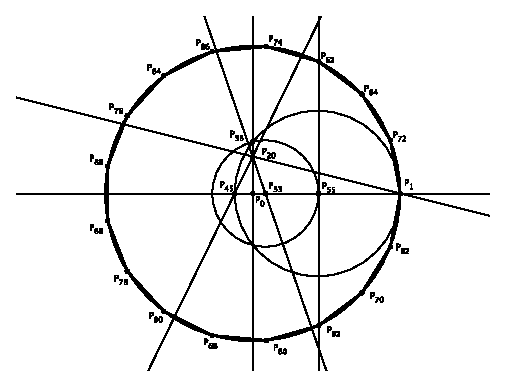
\includegraphics{3_eptadecagon}} 
%\includegraphics{Es1perpendicolare} 
\caption{Costruzione dell'eptadecagono}
\end{center}
\end{figure}


%FINE CAP 3

% LABELS:
%
%\label{potcompl}  prop potenze n-esime di un numero complesso
%\label{osservazionedue}   seconda osservazione par 3.2
%\label{teoremaprimo} Sulla costruibilità per phi
%\label{lemmaprimo}
%\label{lemmasecondo}
%\label{teoremaciclotomia}




%%%%%%%%%%%%%%%%%%%%%%%%%%%%%%%%%%%%%%%%%%%%%%%%%%%%%%%%%%%%%%%%%%%%%%%%%%%%%%%%%%%%%%%%%%%%%%%%%%%%%%%%%%%%%%%%%%%%%%%%%%%%%%%%%%%%%%%%%%%%%%%%%%%%%%%%%%%%%%%%%%%%%%%%





